\documentclass[11pt]{article} 

\hoffset=-.25in
\voffset=-.25in
\oddsidemargin=-.4in
\evensidemargin=0in
\topmargin=-.5in
\textwidth=7.8in
\textheight=8.5in
%\usepackage[a4paper,landscape]{geometry}
\usepackage{amsmath,amsthm,amsfonts,amssymb}
\usepackage{bussproofs}
\usepackage{pdflscape}
\usepackage{hyperref}
\usepackage{booktabs}
\usepackage{subcaption}

\usepackage[parfill]{parskip}

\usepackage{mathtools}
\DeclarePairedDelimiter{\ceil}{\lceil}{\rceil}

\usepackage{algorithm2e}

\usepackage{times}

%%Tikz code%%
\usepackage{tikz}
\usetikzlibrary{arrows,snakes,shapes, decorations.markings}
\tikzset{quartarr/.style={decoration={markings, mark=at position 0.2 with {\arrow[line width=1.5pt]{angle 90}}}, postaction={decorate}}}
\tikzset{midarr/.style={decoration={markings, mark=at position 0.5 with {\arrow[line width=1.5pt]{angle 90}}}, postaction={decorate}}}

\newtheorem{thm}{Theorem}
\theoremstyle{definittion}
\newtheorem{defn}{Definition}

\def\Z{\mathbb Z}
\def\R{\mathbb R}
\def\F{\mathbb F}
\def\C{\mathbb C}
\def\A{\mathbb A}
\def\N{\mathbb N}
\def\Q{\mathbb Q}
%% HoTT shortcuts %%
\def\ctx{\texttt{ctx}}
\def\ap{\texttt{ap}}
\def\pred{\texttt{pred}}
\def\succ{\texttt{succ}}
\def\map{\texttt{map}}
\def\nil{\texttt{nil}}
\def\cons{\texttt{cons}}
\def\List{\texttt{List}}
\def\type{\texttt{Type}}
\def\bool{\texttt{Bool}}
\def\leaves{\texttt{leaves}}
\def\inl{\texttt{inl}}
\def\inr{\texttt{inr}}
\def\0{{\bf 0}}
\def\1{{\bf 1}}
\def\ind{\texttt{ind}}
\def\rec{\texttt{rec}}
\def\refl{\texttt{refl}}
\def\id{\texttt{id}}
\def\db{\texttt{db}}
%\def\span{{\bf span}}
\def\U{\mathcal{U}}
 

\begin{document}



\noindent
{\sffamily  CrySP Research Lab \hfill \bf\sffamily  Cecylia Bocovich}

\bigskip\medskip

\centerline{{\large\bf\sffamily Slitheen Documentation}  \hfill  Last updated: \today}

\section{High Level Overview}


\subsection{Tagging Procedure}

Slitheen uses a tagging procedure very similar to that of Telex~\cite{wustrow2011}, but with a small modification to detect a MiTM or RAD attack. This tagging procedure requires a slight modification to TLSv1.2, outlined as follows:

\begin{figure}[h]
\centering
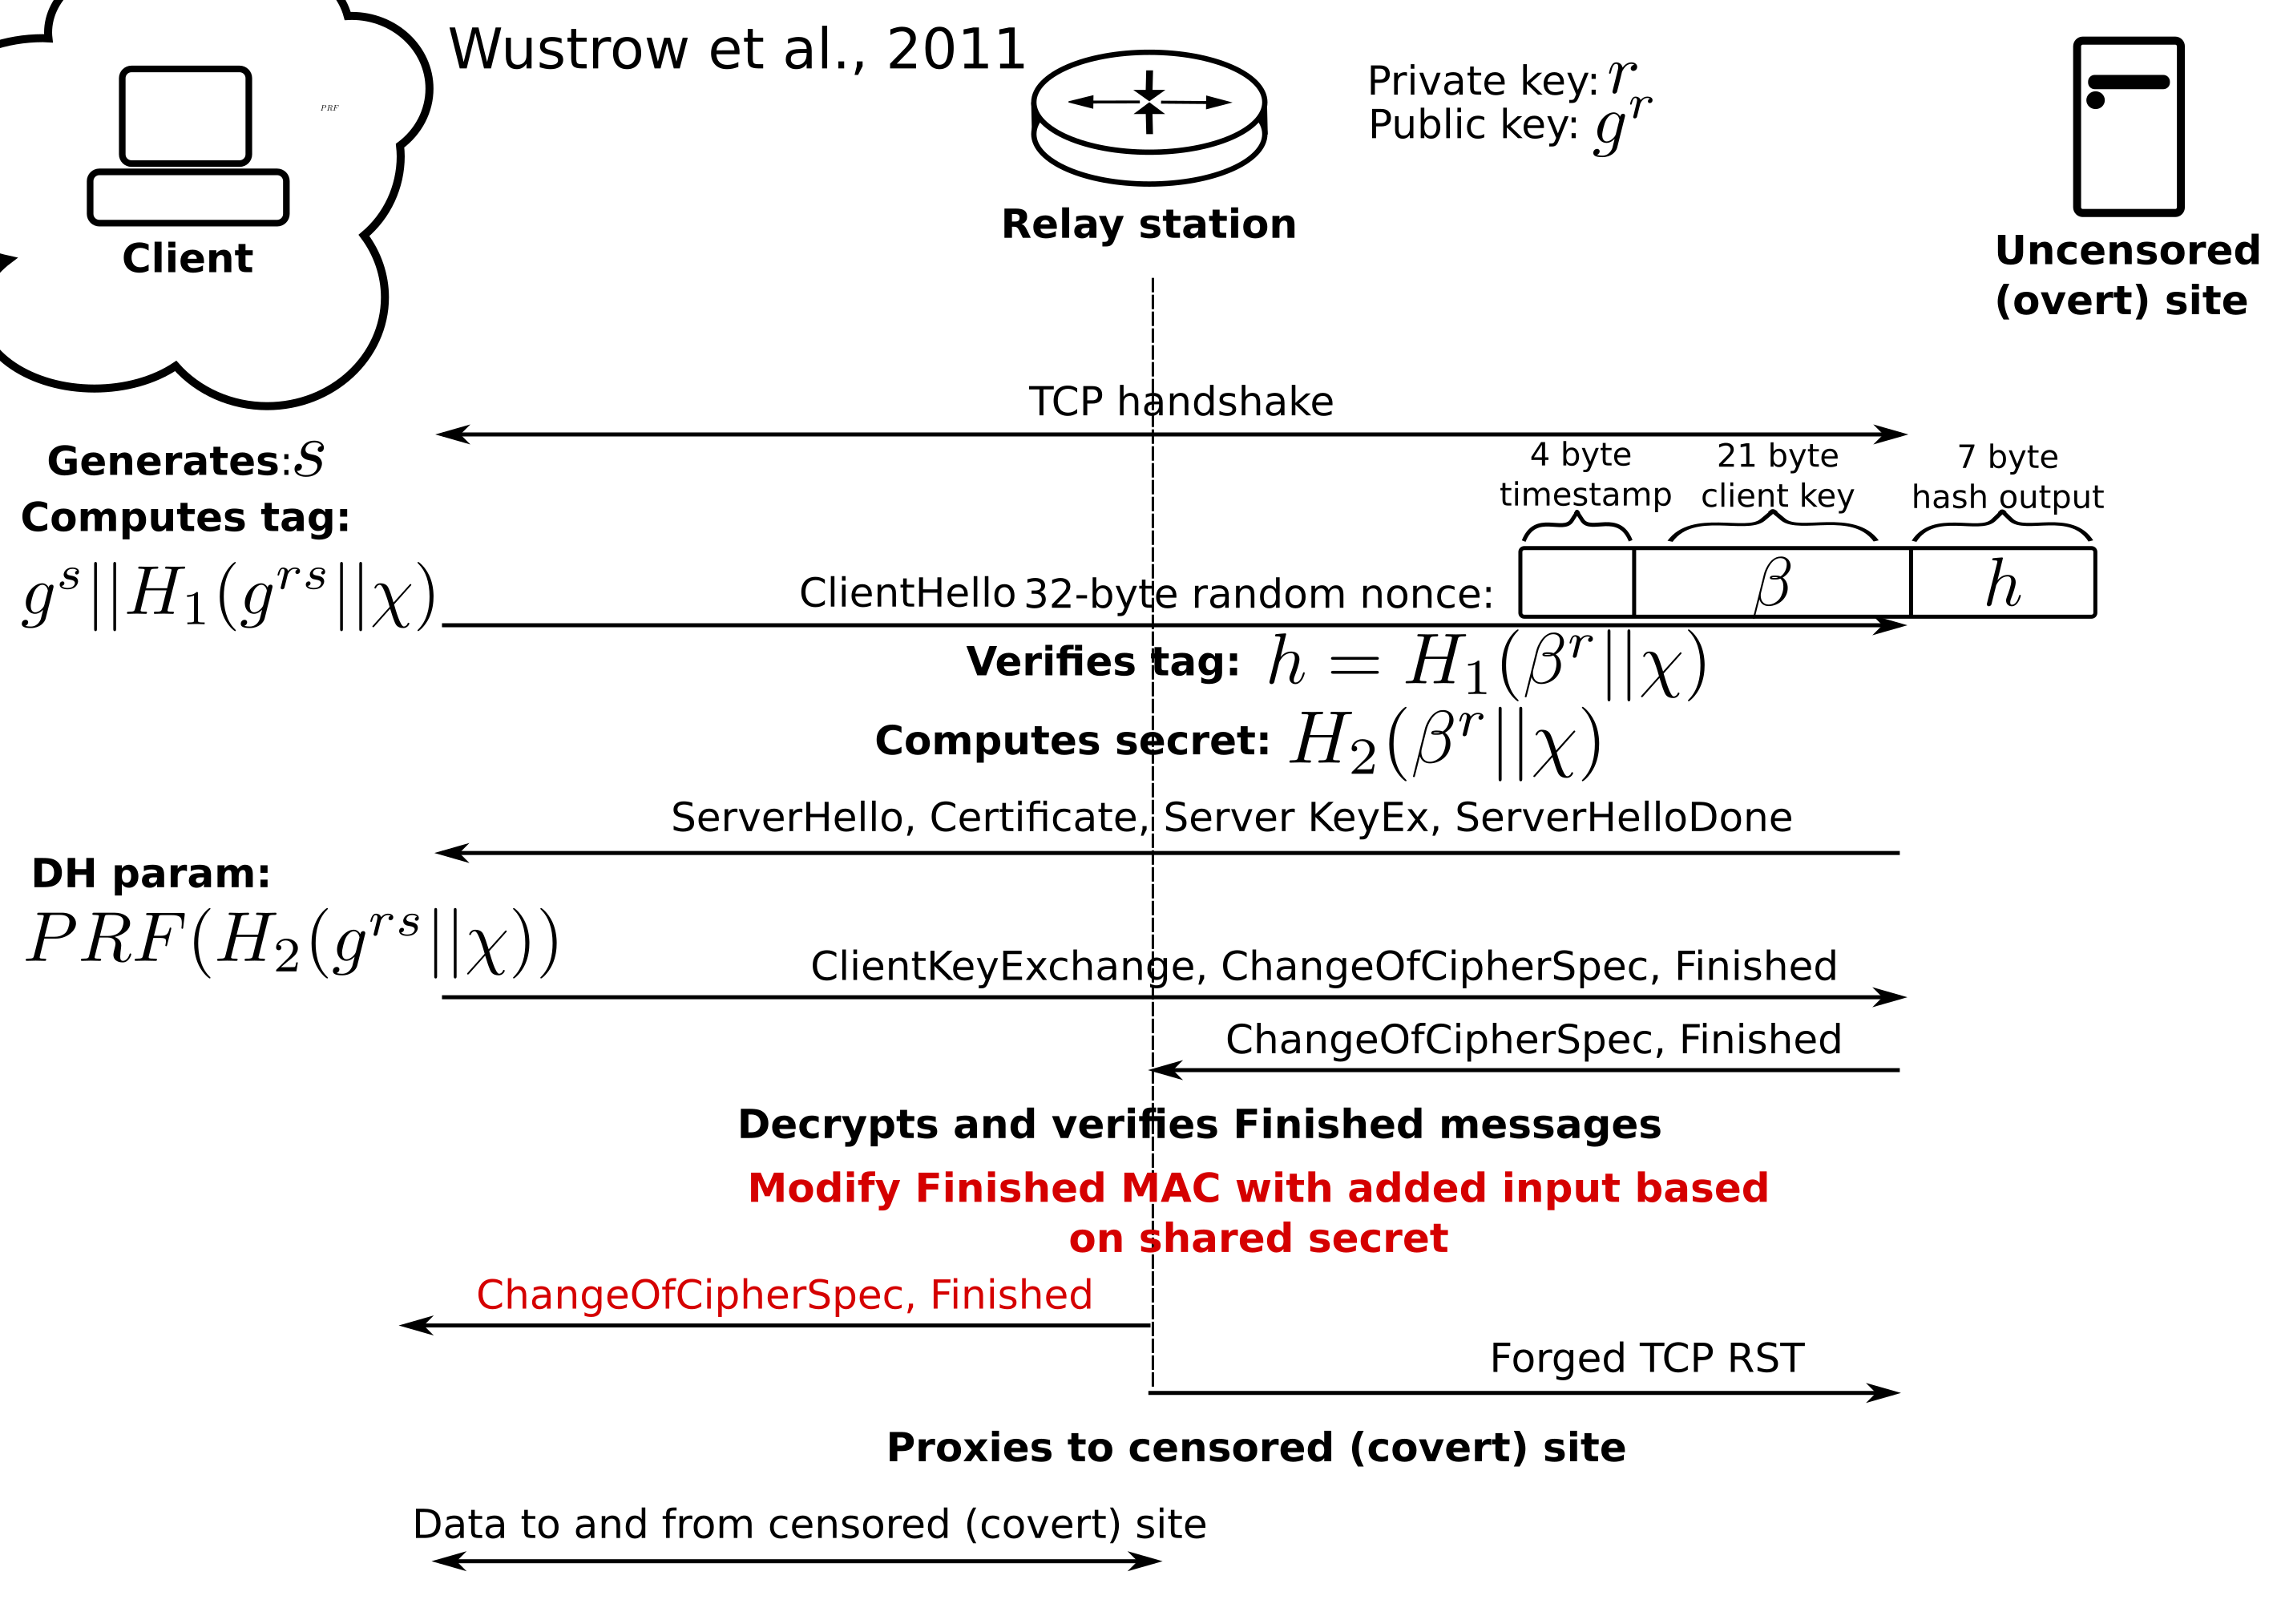
\includegraphics[width=.75\textwidth]{tlsmods}
\caption{Modifications to TLSv1.2 handshake}
\end{figure}

To implement these changes, we have made slight modifications to the OpenSSL source code:

\texttt{git clone -b slitheen git://git-crysp.uwaterloo.ca/openssl}.

These modifications consist mostly of optional callbacks are were made by modifying as little source code as possible, to ease code maintenance.

\subsubsection{Tag generation}

The tag is generated by computing a 21-byte ECDH private key $s$ for the client (along with the corresponding 21-byte public key, $g^s$. We used a custom curve to generate public keys that fit in 21 bytes of the ClientHello random nonce. First, the client randomly chooses between the curve and its twist, in order to maximize the sampling of points that fill the first 21 bytes of the tag. The relay station will check the tag for both the orignal curve and the twist when verifying the tag.

The client's public key is concatenated with a 7-byte value, $H_1(g^{rs} || \chi)$ where $g^{rs}$ is computed by raising the relay station's public key $g^r$ to the client's private key $s$. The context string $\chi$ is just the 4-byte server IP address concatenated with the first 4 bytes of the ClientHello random nonce (in network byte order). The hash function, $H_1$, is the first 7 bytes of SHA256 output, while $H_2$ is the last 16 bytes. The shared secret key between the client and the relay station is computed as $k_{sh} = H_2(g^{rs}||\chi)$.

\subsubsection{DH parameter generation}

To derive the TLS client key exchange parameters, the client computes their secret key as the output of $$PRF_{k_{sh}}(``\texttt{SLITHEEN\_KEYGEN}")$$.

The PRF function here is as defined in the TLSv1.2 RFC\footnote{https://tools.ietf.org/html/rfc5246}, where the hash function used is SHA256 for all cipher suites.

\subsubsection{Modified Finished message}

We change the context of the downstream Finished message, sent from the server to the client. The relay station computes a new Finished message, replacing the previous hash with a MAC keyed with the client-relay shared secret $k_{sh}$:
$$MAC_{k_{sh}}(\texttt{Finished\_hash} || \chi) $$


\subsection{Data Replacement}

Data from the client is modified in both the upstream and downstream direction. Upstream from the client, the client's Slitheen ID along with data to the covert site is included in an additional X-Slitheen header to be extracted and replaced with an X-Ignore header and garbage by the relay station.
Downstream data from the covert site to the client is stored at the relay station until it can be inserted in place of resources that have a leaf content-type (the img supertype).

\subsubsection{Upstream Data from client}

At the start of a flow, the user sends their slitheen ID as the first information in an X-Slitheen header of outgoing HTTP requests. This is followed by a slitheen\_upstream\_header with the stream id of data and the data length. Each stream id indicates a different connection from the client to a covert server.
If a stream is being opened for the first time, the data that follows the slitheen upstream header includes a SOCKS Connect request to the censored site and the first few upstream bytes from the client. Otherwise it includes upstream bytes from the client to be relayed to the censored site. All of the above information is base64 encoded and inserted into an X-Slitheen header.

When the relay station receives the upstream data from a tagged flow, it searches for an X-Slitheen header. If found, it decodes the base64 strings, extracts the information, attributes the flow to the client specified by their slitheen ID.
It then finds connection for the indicated stream or creates a new one and opens a connection the covert site. The station relays data between the client and the covert site by sending bytes through this connection, and saves the responses in a downstream queue for the client specified by the slitheen ID.

When the covert site responds with information, this data is stored in blocks at the relay station as part of the client's downstream queue. Each block contains information about the stream ID, and the length of the block.

\subsubsection{Downstream Data to client}

When resources come back from the overt site, they are decrypted when allowed, and their content type and length is stored in the HTTP state of the flow. To fill the contents of a packet of length $n$, the relay station determines the HTTP state, the content type of the resource, and the garbage bytes needed to pad the AES-CBC encrypted data.

The relay station then updates the HTTP state of the flow and processes the next packet.

\section{Protocol Details}

\subsection{TLS v1.2 Handshake Modifications}

Slitheen uses a slightly modified TLS handshake, similar to Telex~\cite{wustrow2011}. In order to properly process handshake messages, the relay must reconstruct them before processing. In the case of all messages preceding the Finished message, this can be done without blocking. Since we are modifying the Finished message hash, this message must be held at the station until it is reconstructed, verified, and replaced.

We fully support session resumption through session IDs and session tickets. The state machine for the relay station is very similar to the OpenSSL state machine, I will only describe here the modifications we make.

We assume that the relay station has generated an elliptic curve public-private key pair $(r, g^r)$, and has distributed its public key, $g^r$, to the client. %TODO: include details on curve

Definitions for PRF and unaltered handshake messages are as defined in RFC 5246~\cite{rfc5246}.

\subsubsection{Client}

The states we care about for the client are:
\begin{itemize}
\item SEND\_CLNT\_HELLO
\item SEND\_CLNT\_KEY\_EXCHANGE
\item RECV\_SRVR\_FINISHED
\item SEND\_CLNT\_FINISHED
\end{itemize}

\textbf{SEND\_CLNT\_HELLO}

A client first generates an elliptic curve public-private key pair $(s, g^s)$.

When the client sends the ClientHello message, they replace the 32-byte random nonce with their elliptic curve pubic key point and a verification hash. These values concatenated comprise a 28-byte \emph{tag}.

\begin{figure}[h]
\begin{subfigure}{\textwidth}
\centering

\includegraphics{old_client_hello}
\caption{Original TLS CientHello random nonce}

\end{subfigure}

\vspace{5mm}
\begin{subfigure}{\textwidth}
\centering

\includegraphics{new_client_hello}
\caption{Modified (tagged) TLS CientHello random nonce}

\end{subfigure}
\caption{Modifications to the ClientHello message}
\end{figure}

The client then computes a shared secret with the relay station of the form $g^{rs}$. The 7-byte verification hash is the first 56 bits of SHA$256(g^{rs||\chi})$ where $\chi = $ \texttt{server\_ip||UNIX\_timestamp||TLS\_session\_id}.

\textbf{SEND\_CLNT\_KEY\_EXCHANGE}

The client computes their key exchange parameters from the shared secret with the relay station. In particular, their private key is the output of a PRF on the client-relay shared secret $h^{rs}$, and a constant string.

For example, in a ciphersuite using EDH or ECDH, the client generates their private key as follows:
$$a = \texttt{PRF}(h^{rs} || \texttt{"SLITHEEN\_KEYGEN"})$$

Afterwards, $h^a$ is sent to the server in the usual manner.

\textbf{RECV\_SRVR\_FINISHED}

The client should verify the Finished MAC of the server's Finished message after decrypting it. The MAC can be of one of two possible acceptable forms:
\begin{enumerate}
\item The usual PRF output of the hashed, previously seen handshake messages:
$$\texttt{Finished\_MAC} = \texttt{PRF}(\texttt{FINISHED\_CONST}||\texttt{Hash(handshake\_messages}))$$
\item A modified MAC with an extra input (based on the client-relay shared secret) hashed in with the handshake messages:
$$\texttt{extra\_input} = \texttt{PRF}(g^{rs} || \texttt{"SLITHEEN\_FINISH"})$$

$$\texttt{Finished\_MAC} = \texttt{PRF}(\texttt{FINISHED\_CONST}||\texttt{Hash(handshake\_messages} || \texttt{extra\_input}))$$

\end{enumerate}

If the client receives the first hash, it should proceed loading the page, but not use the session for decoy routing. The receipt of a normal finished message indicates possible problems with the relay station, a MiTM attack, or a RAD attack.

If the client receives the second hash, it knows that the relay station has intercepted the flow and it is safe to use for decoy routing.

\textbf{SEND\_CLNT\_FINISHED}

The client should send a Finished message back to the server with the previously seen messages hashed into the Finished messages hash, with one exception. The client should compute the MAC expected from the server, before modification by the relay station (MAC 1 above). A Finished message with this MAC should be hashed into the client's Finished message MAC instead of the one the client received.

\subsubsection{Relay Station}

Upon receipt the receipt of any handshake message, the relay station hashes it into it's Finished MAC computation. Additionally, if the ClientHello and ServerHello messages indicate a session resumption, the relay station computes the Finished message MACS and reads the TLS master secret for the session from the new random nonces and its saved session store, respectively.

The states we care about for the relay are:
\begin{itemize}
\item RECV\_CLNT\_HELLO
\item RECV\_SRVR\_KEY\_EXCHANGE
\item RECV\_SRVR\_FINISHED
\item RECV\_CLNT\_FINISHED
\end{itemize}


\textbf{RECV\_CLNT\_HELLO}

When the relay station receives a ClientHello message from any client, it first checks to see if the random nonce is tagged. To do so, it extracts the client's 21-byte public key, $g^s$, and computes the shared secret $g^{sr} = g^{rs}$. It uses this value to compute the verification hash SHA$256(g^{rs||\chi})$ and checks this against the last 7 bytes of the random nonce. If the two values are equal, the relay station saves the shared key and flow information (ip addresses and port numbers) to identify later handshake messages in the same flow.

\textbf{RECV\_SRVR\_KEY\_EXCHANGE}

Upon receipt of the server key exchange parameters, the relay station is able to compute the TLS master secret. Since the client's private key is computed from the client-relay shared secret, the relay station can compute the client's private key parameter:

$$a = \texttt{PRF}(g^{rs} || \texttt{"SLITHEEN\_KEYGEN"})$$

The server's public key, $h^b$, along with the client's private key $a$ allows the relay station to compute the TLS master secret:
$$\texttt{master\_secret} = \texttt{PRF} (h^{ab} || \texttt{MASTER\_SECRET\_CONST} || \texttt{client\_random} || \texttt{server\_random})$$

\textbf{RECV\_SRVR\_FINISHED}

When the relay station receives an encrypted Finished message for a tagged flow, it should have already computed the TLS master secret for the flow.
The relay station then attempts to decrypt the Finished message.
If the decryption was unsuccessful, the relay station removes the flow from its memory and forwards the message to the client unchanged.

If the decryption was successful, the relay station verifies the Finish message hash with against the handshake messages seen so far. If the hash doesn't equal what the relay station expects, the flow is removed from its memory and the message is forwarded unchanged.

%TODO: update with new method, when implemented
If the Finished message verifies correctly, the relay station replaces it with a different, modified hash. It feeds the output of a PRF seeded with the client-relay shared secret and a constant into the Finished hash computation and computes the final MAC for the Finished message. The purpose of this step is to alert the client to the fact that the flow has been successfully tagged and intercepted by a relay station. The Finished MAC sent to the client is computed as follows:

$$\texttt{extra\_input} = \texttt{PRF}(g^{rs} || \texttt{"SLITHEEN\_FINISH"})$$

$$\texttt{Finished\_MAC} = \texttt{PRF}(\texttt{FINISHED\_CONST}||\texttt{Hash(handshake\_messages} || \texttt{extra\_input}))$$

\textbf{RECV\_CLNT\_FINISHED}

The relay station should verify that the client's Finished message MAC contains a hash of all handshake messages seen so far (without the addition of the extra input based on the client-relay shared secret).


\subsection{Upstream Application Data (Client $\rightarrow$ Covert)}

SOCKS data from the client to the covert site is sent in upstream slitheen blocks. These blocks contain a 4-byte header that indicates the 2-byte stream ID of the data (which SOCKS connection it belongs to), and the length.

\subsubsection{client}
When the client first starts a new browsing session, they generate a 28-byte slitheen\_ID. This ID is sent to the Overt User Simulator (OUS) to be included in the X-Slitheen header of every outgoing HTTP request from the client to the overt server in a tagged flow.

When the client's browser requests a new connection, the SOCKS frontend generates a new stream ID for that connection. It then sends the SOCKS connect request and upstream bytes from the client to the relay station in base64-encoded upstream slitheen blocks to the OUS. The OUS then sends these space-delimited, encoded blocks in the X-Slitheen header of outgoing overt HTTP requests, along with the client's slitheen\_ID. 

\subsubsection{relay}

Upon receiving a new HTTP request from the client, the relay station decrypts the request and searches for an X-Slitheen header. The contents of this header include a series of space-delimited base64 encoded strings. The relay station decodes the strings to retrieve the client's slitheen\_ID and the upstream slitheen blocks containing SOCKS data.

At this point, the relay station can associate the flow with the client's slitheen\_ID and corresponding downstream data queue.

If the blocks contain a SOCKS connect request for a new stream, the relay station spins off a new thread for that stream and makes a TCP connection to the covert server. It then sends the SOCKS data from the client through this connection and saves the covert site's responses in the downstream data queue indicated by the client's slitheen\_ID.

The relay station should then replace the X-Slitheen header with an X-Ignore header and garbage bytes to protect the client's identity and browsing habits.

\subsection{Downstream Application Data (Covert $\rightarrow$ Client)}

SOCKS data from the covert site is delivered to the client (according to the slitheen\_ID of the flow) in downstream slitheen blocks. Each slitheen block contains a 16-byte header containing the stream ID of the data, a counter to indicate the order of blocks in the same stream, the length of SOCKS data, the length of garbage bytes, and a padding of zeros. This header is AES encrypted in ECB mode with a key generated from the slitheen\_ID. The body of the slitheen block is AES encrypted in CBC mode with a key generated as a part of the same key block:
$$\texttt{slitheen\_key\_block} = \texttt{PRF}(\texttt{slitheen\_ID}) || \texttt{"SLITHEEN\_SUPER\_ENCRYPT"})$$
$$\texttt{slitheen\_header\_key} = \texttt{slitheen\_key\_block}[0:\texttt{key\_len}-1] $$
$$\texttt{slitheen\_body\_key} = \texttt{slitheen\_key\_block}[\texttt{key\_len}:2\texttt{key\_len}-1] $$

If there are any bytes in the packet left over after reducing the size to fit in 16-byte blocks, this is filled with randomly generated garbage bytes and the garbage length field in the downstream slitheen header is set to reflect the amount of garbage padding.
A block that contains only garbage indicates that there was no downstream data for the client queued at the relay station.

\begin{figure}[h]
\begin{subfigure}{\textwidth}
\centering

\includegraphics[width=.75\textwidth]{downstream_slitheen_header}
\caption{Header for downstream slitheen blocks}
\end{subfigure}

\vspace{5mm}

\begin{subfigure}{\textwidth}
\centering

\includegraphics[width=.75\textwidth]{downstream_slitheen_block}
\caption{Full, encrypted downstream slitheen block}
\end{subfigure}
\caption{Format of SOCKS data from the covert site to the client, injected in the place of leaf resources}

\end{figure}

\subsubsection{client}

When the client's Overt User Simular (OUS) receives a resource of Content-Type slitheen, it sends the length of the resource and the HTTP response body to the client's SOCKS proxy front-end to be parsed and sent to the client's browser. 

The SOCKS proxy frontend parses these resources to extract downstream slitheen blocks. After receiving the resource length, it parses downstream slitheen blocks one-by-one, first decrypting the header to determine the length, then decrypting the slitheen block body to retrieve the SOCKS data. The SOCKS proxy then writes this data to the browser, using the connection indicated by the stream ID in the header. The proxy skips garbage bytes, and moves on to decrypting the next downstream slitheen block.

It is possible for downstream slitheen blocks to arrive in a resource out of order. If this happens, the SOCKS proxy should consult the counter field of the header and hold premature blocks until their predecessors have arrived before writing data to the browser.

The SOCKS proxy front-end should also verify the zero padding at the end of the downstream header.

\subsubsection{relay}
The relay station saves the TLS record and HTTP state of each flow to determine when the contents of packets from the server to the client can be replaced. The goal is to only replace the body of HTTP responses with a leaf content type, and to change the content type in the header to ``slitheen''. Replaced content is contained in downstream slitheen blocks.

\texttt{Content-Type: slitheen}

A flow can be in one of three TLS record states when a new packet is received:
\begin{itemize}
\item BEGIN\_RECORD
\item MID\_RECORD
\item END\_RECORD
\end{itemize}

If the packet contains an entire TLS record, this record can be decrypted and used to update the HTTP state of the flow.

A flow can be in one of 7 HTTP states when a new packet is received:
\begin{itemize}
\item BEGIN\_HEADER
\item MID\_HEADER
\item BEGIN\_CHUNK
\item MID\_CHUNK
\item END\_CHUNK
\item RESPONSE\_BODY
\item UNKNOWN
\end{itemize}

\textbf{BEGIN\_HEADER and MID\_HEADER}

The header of an HTTP response must be decrypted to determine the HTTP state of the flow in future packets. The header contains the content-type of the response and the length of the response, specified either in chunks as indicated by the transfer encoding header or in the content length header field.

Upon receiving and decrypting an HTTP response header, the relay station should determine the value of the Content-Type header. If it is a leaf content type (e.g., ``image/*'' or ``text/plain''), the relay station should change the value of Content-Type to ``slitheen'' (padded with spaces to preserve length). The length/transfer encoding of the response is then saved in the flow's state.

An HTTP header ends with the string ``CR LF CR LF''.

\textbf{BEGIN\_CHUNK}

If the transfer encoding is chunked, the length of the response is determined by the length of each chunk received. Each chunk begins with a string indicating the length and a newline ``[length] CR LF''. When a new chunk begins, the relay station must decrypt the length to determine the number of bytes in subsequent records that belong to the chunk, before the next chunk begins.

\textbf{MID\_CHUNK and RESPONSE\_BODY}

In the middle of a chunk (or in the response body for resources whose length is specified by the Content-Length header), records can be replaced with downstream content without being decrypted. If a record is longer than the received packet, the relay station should calculate an entire record's worth of encrypted downstream content. 

If a newly received record is longer than the packet and the remaining chunk or response body length, the relay station will be unable to properly calculate the entire record. In this case, the relay station should forward the record unchanged, leaving the client's SOCKS5 frontend to parse only legitimate slitheen blocks.

\textbf{END\_CHUNK}

In a transfer-encoded resource, chunks are terminated with a ``CRLF'' before ending the stream or beginning a new chunk. The relay station should verify a chunk has ended by checking for this string. Failure to verify this could indicate that a problem occurred with the HTTP state calculation.

\textbf{UNKNOWN}

A flow's HTTP state can become unknown in the following cases:
\begin{itemize}
\item The relay station received a record too big to decrypt while in the PARSE\_HEADER or MID\_HEADER states.
\item The relay station received a record too big to decrypt that extended past the end of a resource while in the MID\_CHUNK or RESPONSE\_BODY states.
\end{itemize}

A flow can recover from this unknown state by saving the contents of seen packets and parsing them after-the-fact. Knowledge of the state will likely come too late to replace the resource, but may be useful if more than one resource is sent in a single flow.

\begin{figure}[h]
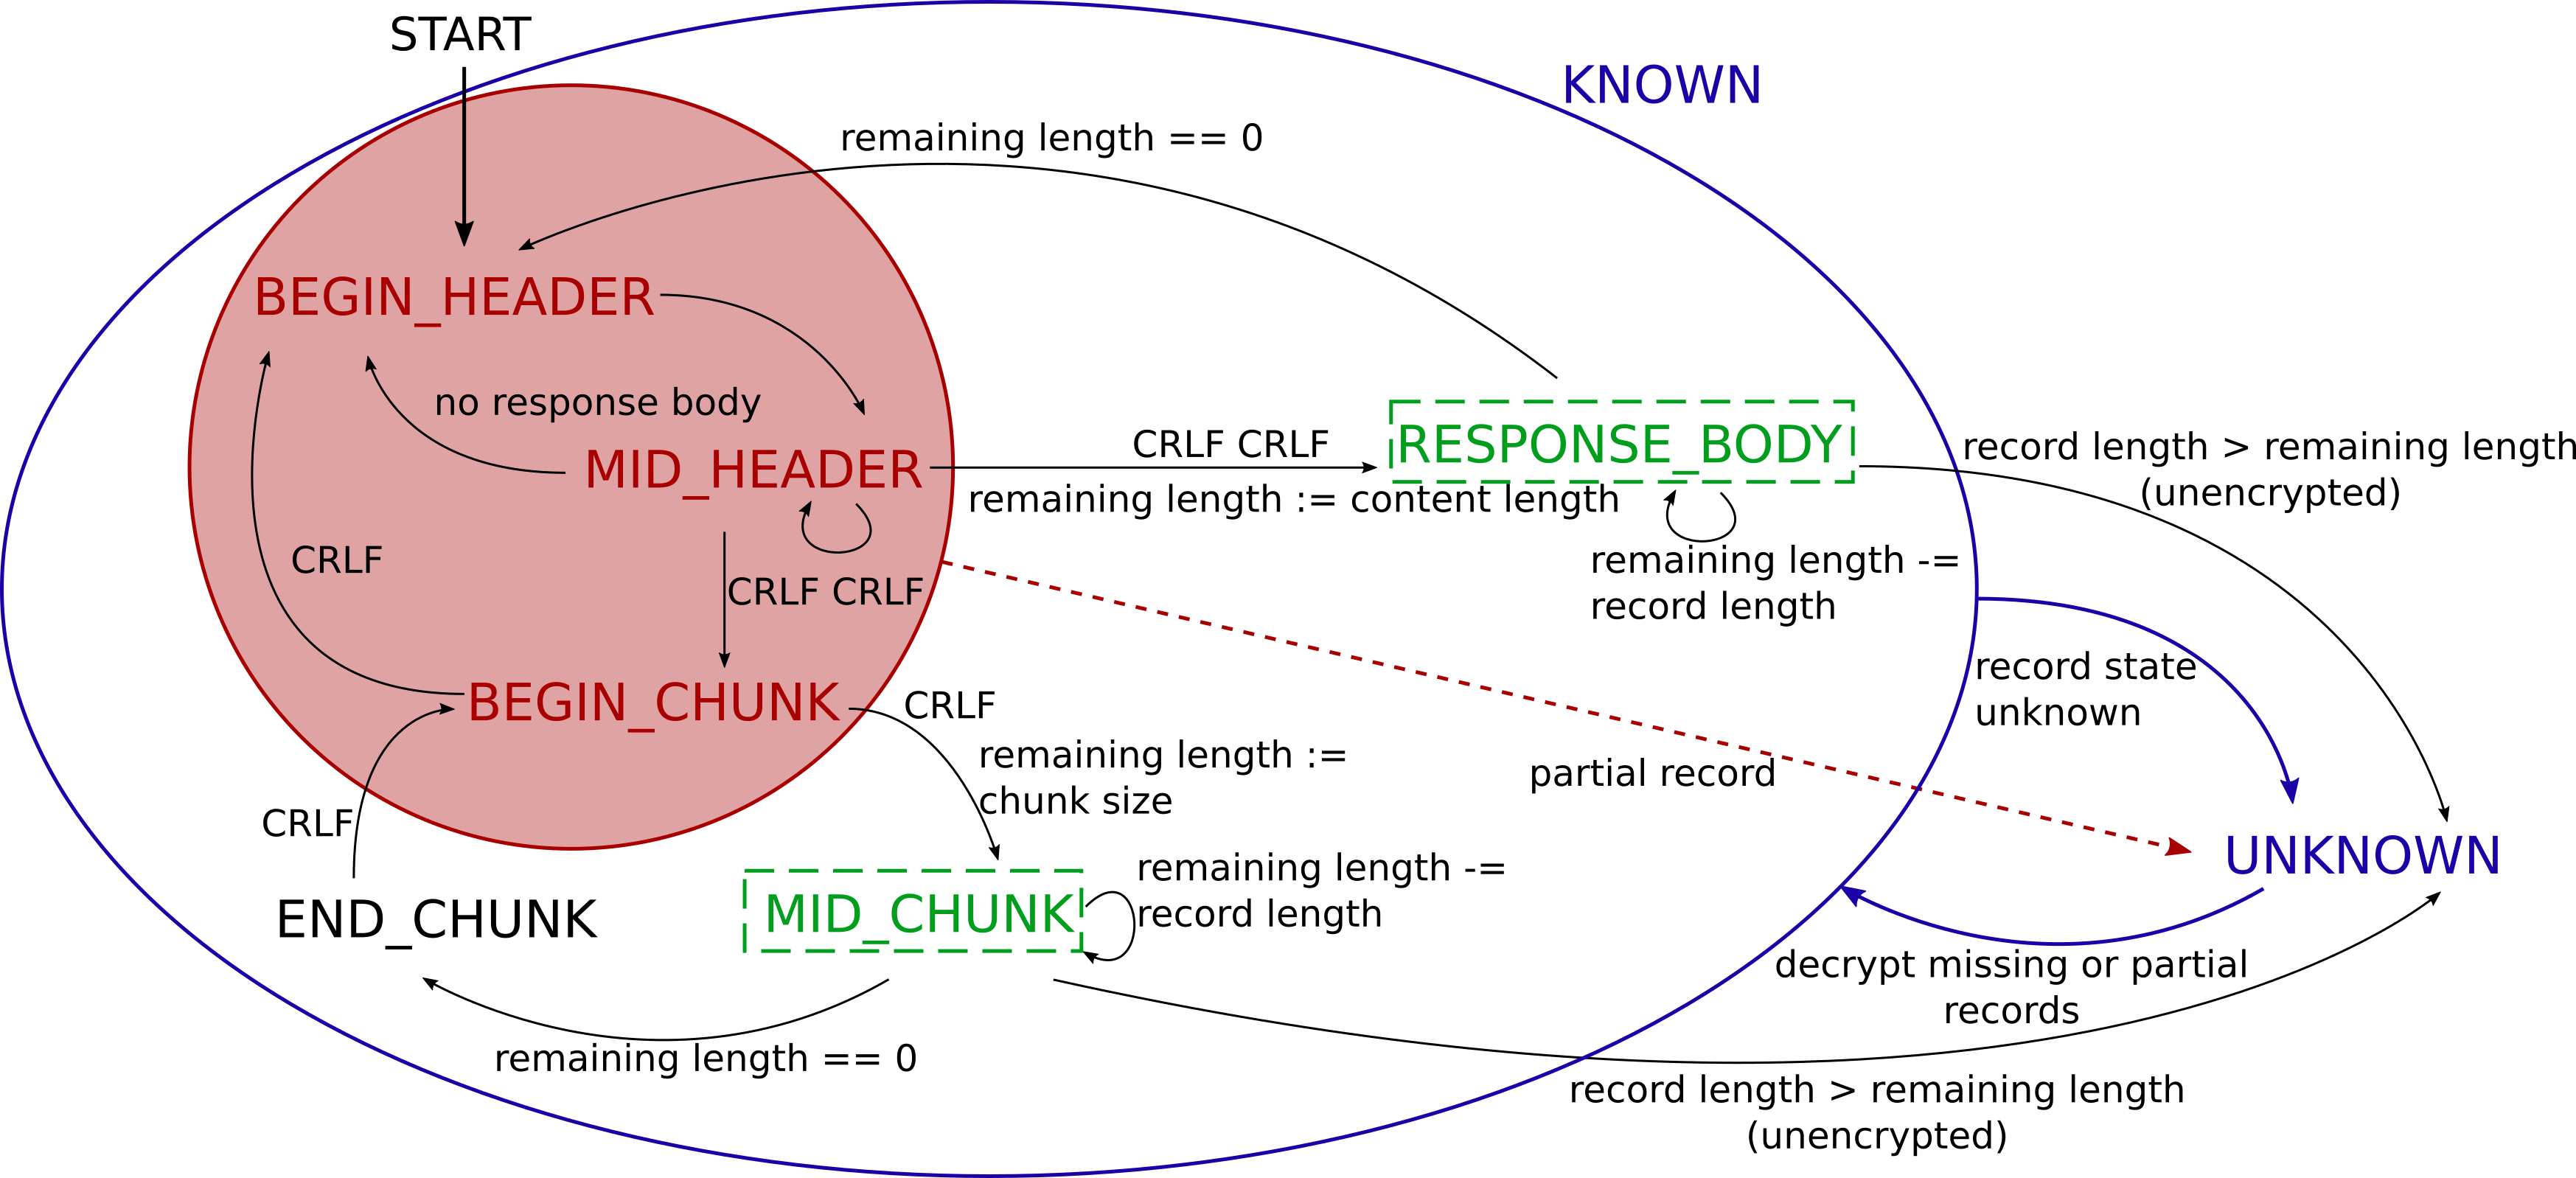
\includegraphics[width=\textwidth]{httpstate}
\caption{State machine of HTTP states for a tagged flow. Packets received in a green state can be replaced without decrypting the TLS record. At a red state, an incoming record must be entirely contained in the packet contents and decrypted to determine future states of the flow and use the resource for downstream data. Failure to decrypt a record in a red state will result in an unknown HTTP state for the flow.}
\end{figure}


\nocite{*}

\bibliographystyle{abbrv}
\bibliography{documentation} 
\end{document}
